\documentclass[a4paper,12pt]{article}

\usepackage[utf8]{inputenc}
\usepackage[T1]{fontenc}
\usepackage[english,french]{babel}
\usepackage{graphicx}
\usepackage{amsmath,amssymb}
\usepackage{geometry}
\geometry{a4paper, margin=1in}

\title{Rapport de Projet}
\author{MARIAC Damien, LABOURAIL Célia , GERMAIN Marine,
EL SAWADOGO Kader}


\begin{document}

\maketitle

\begin{abstract}
Ce document présente le rapport du projet réalisé dans le cadre du cours d'application statistique. Il détaille les objectifs, la méthodologie, les résultats obtenus et les conclusions tirées.
\end{abstract}


\tableofcontents

\newpage

\section{Contexte et Objectifs Marine}

\newpage

\section{Méthodologie Damien}

\newpage

\section{Forces et Faiblesses Célia}

\newpage

\section{Exemples d'applications Kader}

\newpage

\section{BRAIN STORM --------------------}

\section{Les différentes méthodes}
\subsection{Méthodes au niveau des données}
Les méthodes data-level agissent directement sur les données d’entraînement pour atténuer le
déséquilibre entre classes. Le principe est soit d’augmenter le poids de la classe minoritaire en lui
fournissant plus d’exemples (réels ou synthétiques), soit au contraire de réduire le poids de la classe
majoritaire en éliminant certains de ses exemples. L’objectif est d’obtenir une distribution de classes
plus équilibrée, ce qui force l’algorithme d’apprentissage à prêter autant d’attention à la minorité qu’à la
majorité. Ces techniques peuvent toutefois introduire de la variance (sur-apprentissage) ou du
biais supplémentaire, il faut donc les appliquer judicieusement.

\subsubsection{Sur-échantillonnage (Over-sampling)}

Le sur-échantillonnage (oversampling) consiste à ajouter des copies ou des variantes des exemples de
la classe minoritaire jusqu’à augmenter sa fréquence dans le jeu de données. Dans sa forme la plus
simple, le sur-échantillonnage aléatoire (Random Over-Sampling, ROS) duplique aléatoirement des
instances minoritaires existantes jusqu’à atteindre un équilibre désiré. Par exemple, si l’on dispose
de 100 exemples minoritaires et 1000 majoritaires, le ROS peut répliquer les minoritaires
(éventuellement plusieurs fois chacun) jusqu’à en obtenir 1000, rétablissant ainsi un ratio équilibré. On échantillonne avec remise parmi les indices de la classe minoritaire pour
générer de nouvelles instances d’entraînement.

\subsubsection{Sous-échantillonnage (Under-sampling)}

À l’inverse, le sous-échantillonnage (undersampling) vise à réduire la proportion de la classe
majoritaire en retirant certains de ses exemples du jeu de données. Le sous-échantillonnage aléatoire
(Random Under-Sampling, RUS) élimine au hasard des instances de la classe majoritaire jusqu’à atteindre
un ratio plus équilibré avec la minorité.le RUS est utile lorsque l’on dispose d’une grande abondance de
données majoritaires, potentiellement redondantes. Plutôt que de tout utiliser, ce qui peut être
coûteux et inutile, on peut se permettre d’en élaguer une partie. En réduisant drastiquement le nombre
d’exemples majoritaires, on élimine le biais numérique et on accélère l’entraînement (moins de
données à parcourir).

\subsubsection{SMOTE (Synthetic Minority Over-sampling Technique)}



Plutôt que de copier des instances existantes,
SMOTE crée de nouvelles instances minoritaires artificielles en interpolant entre des exemples réels.Concrètement, pour chaque exemple minoritaire original, SMOTE sélectionne aléatoirement l’un de ses
$k$ plus proches voisins (minoritaire également), puis génère un nouvel exemple situé aléatoirement le
long du segment joignant les deux points dans l’espace des \textit{features}. En répétant ce procédé, on
peut synthétiser autant d’exemples minoritaires que souhaité.



\subsection{Méthodes au niveau de l'algorithme }
????????





\newpage

\section*{Annexe}

\begin{figure}[h!]
    \centering
    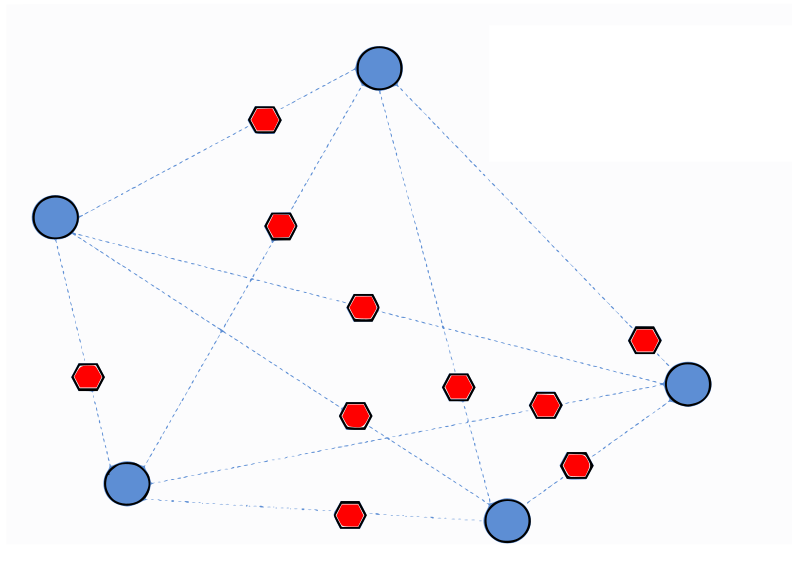
\includegraphics[width=0.8\textwidth]{images/smote.png}
    \caption{Smote illustration}
    \label{fig:example}
\end{figure}
Les points bleu correspondent à la classe minoritaire dont on souhaite générer de nouveaux exemples, les points rouge sont les points générés par SMOTE.


\newpage
\section*{bibliographie}

\end{document}